
\section{Experimental Setting}\label{sec:experiments}

Now that we have introduced the theoretical distinctions between the multi-armed bandit (MAB) algorithms EXP3, EXP3E, and our proposed LinEXP3E in the previous section, we shift toward empirical validation. This section presents the experimental setup and results used to evaluate LinEXP3E in a contextual bandit environment. The goal of our experiments was to assess the algorithm's learning behavior, regret performance \ref{eq:regret}, and causal inference capabilities, in particular its ability to estimate average treatment effect (ATE) \ref{eq:ate} between arms using inverse propensity weighting (IPW). Through a series of simulations, we aim to demonstrate that LinEXP3E maintains a strong exploration-exploitation trade-off as well as supports reliable estimation.

We begin by describing the simulation environment and evaluation metrics. Following that, we present empirical results in terms of cumulative reward, regret trends, and ATE convergence, both with and without IPW.

\\
We evaluate LinEXP3E in a contextual bandit environment with $K = 5$ arms. Each arm is associated with a true but unknown reward vector $\theta_a \in \mathbb{R}^{10}$, where $10$ is the context dimensionality. $\theta_a$ is randomly initialized at the start of the simulation. At each time step $t$, the agent receives a context vector $x_t \sim \mathcal{N}(0, I_{d})$ where $d=10$ and selects an arm $a_t \in \mathcal{A}$ based on a softmax-style policy distribution.

The observed reward is generated according to a linear model with Gaussian noise:
\[
r_t = \langle x_t, \theta_{a_t} \rangle + \epsilon_t, \quad \epsilon_t \sim \mathcal{N}(0, 0.1^2)
\]
The algorithm runs for $T = 1000$ rounds. We set the number of MGR samples to $M = 10$ and the exploration parameter $\gamma = 0.1$.

We track cumulative reward, average regret, and average treatment effect per each arm combination. 

\subsection{Results}\label{subsec:results}

The following graphs summarize our empirical findings. The plots generated during simulation illustrate the algorithm's improving reward and sublinear cumulative regret, as well as the convergence behavior of the ATE pairwise comparisons.

\begin{figure}[H]
\centering
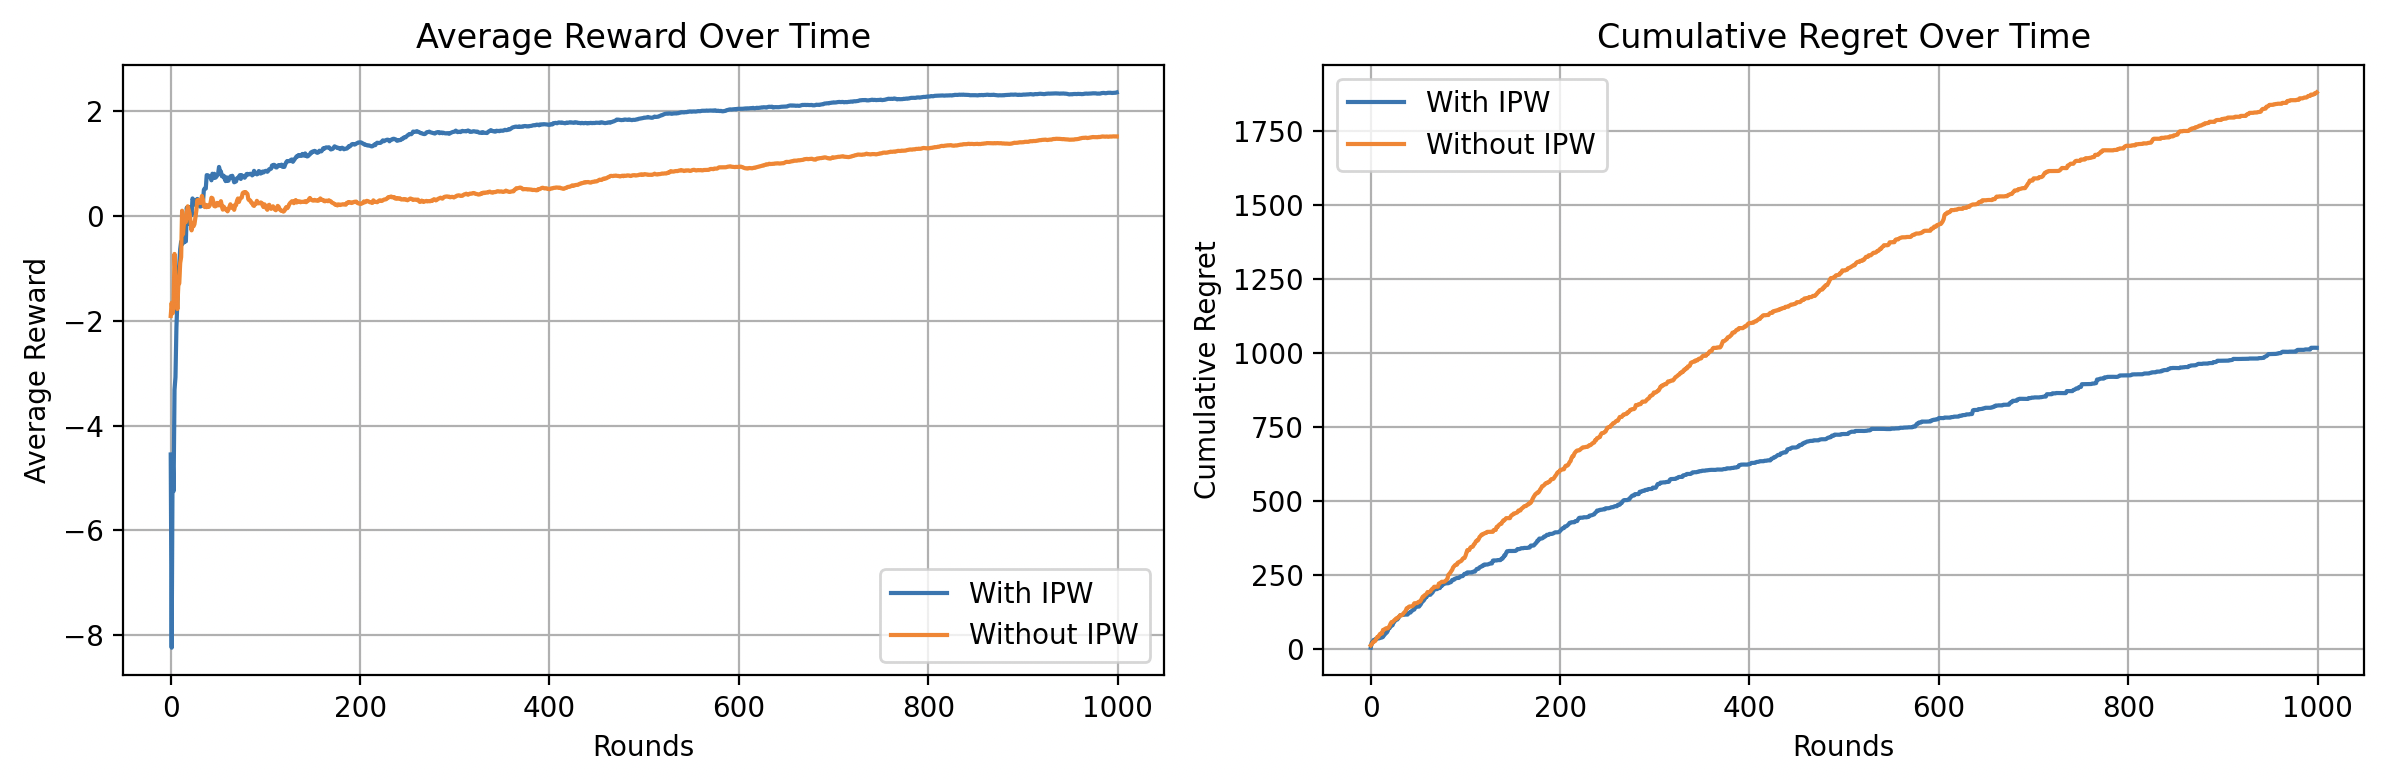
\includegraphics[width=0.9\textwidth]{performance_comparing_ate.png}
\caption{(Left) Average Reward over Time. (Right) Cumulative Regret over Time.}
\label{fig:reward_regret}
\end{figure}

Figure~\ref{fig:reward_regret} shows that the algorithm’s average reward increases over time as it learns to select higher-reward arms, while cumulative regret grows sublinearly, suggesting effective balancing of exploration and exploitation. We compare these reward and regret measures according to their incorporation of inverse propensity weighting (IPW).

\begin{figure}[H]
\centering
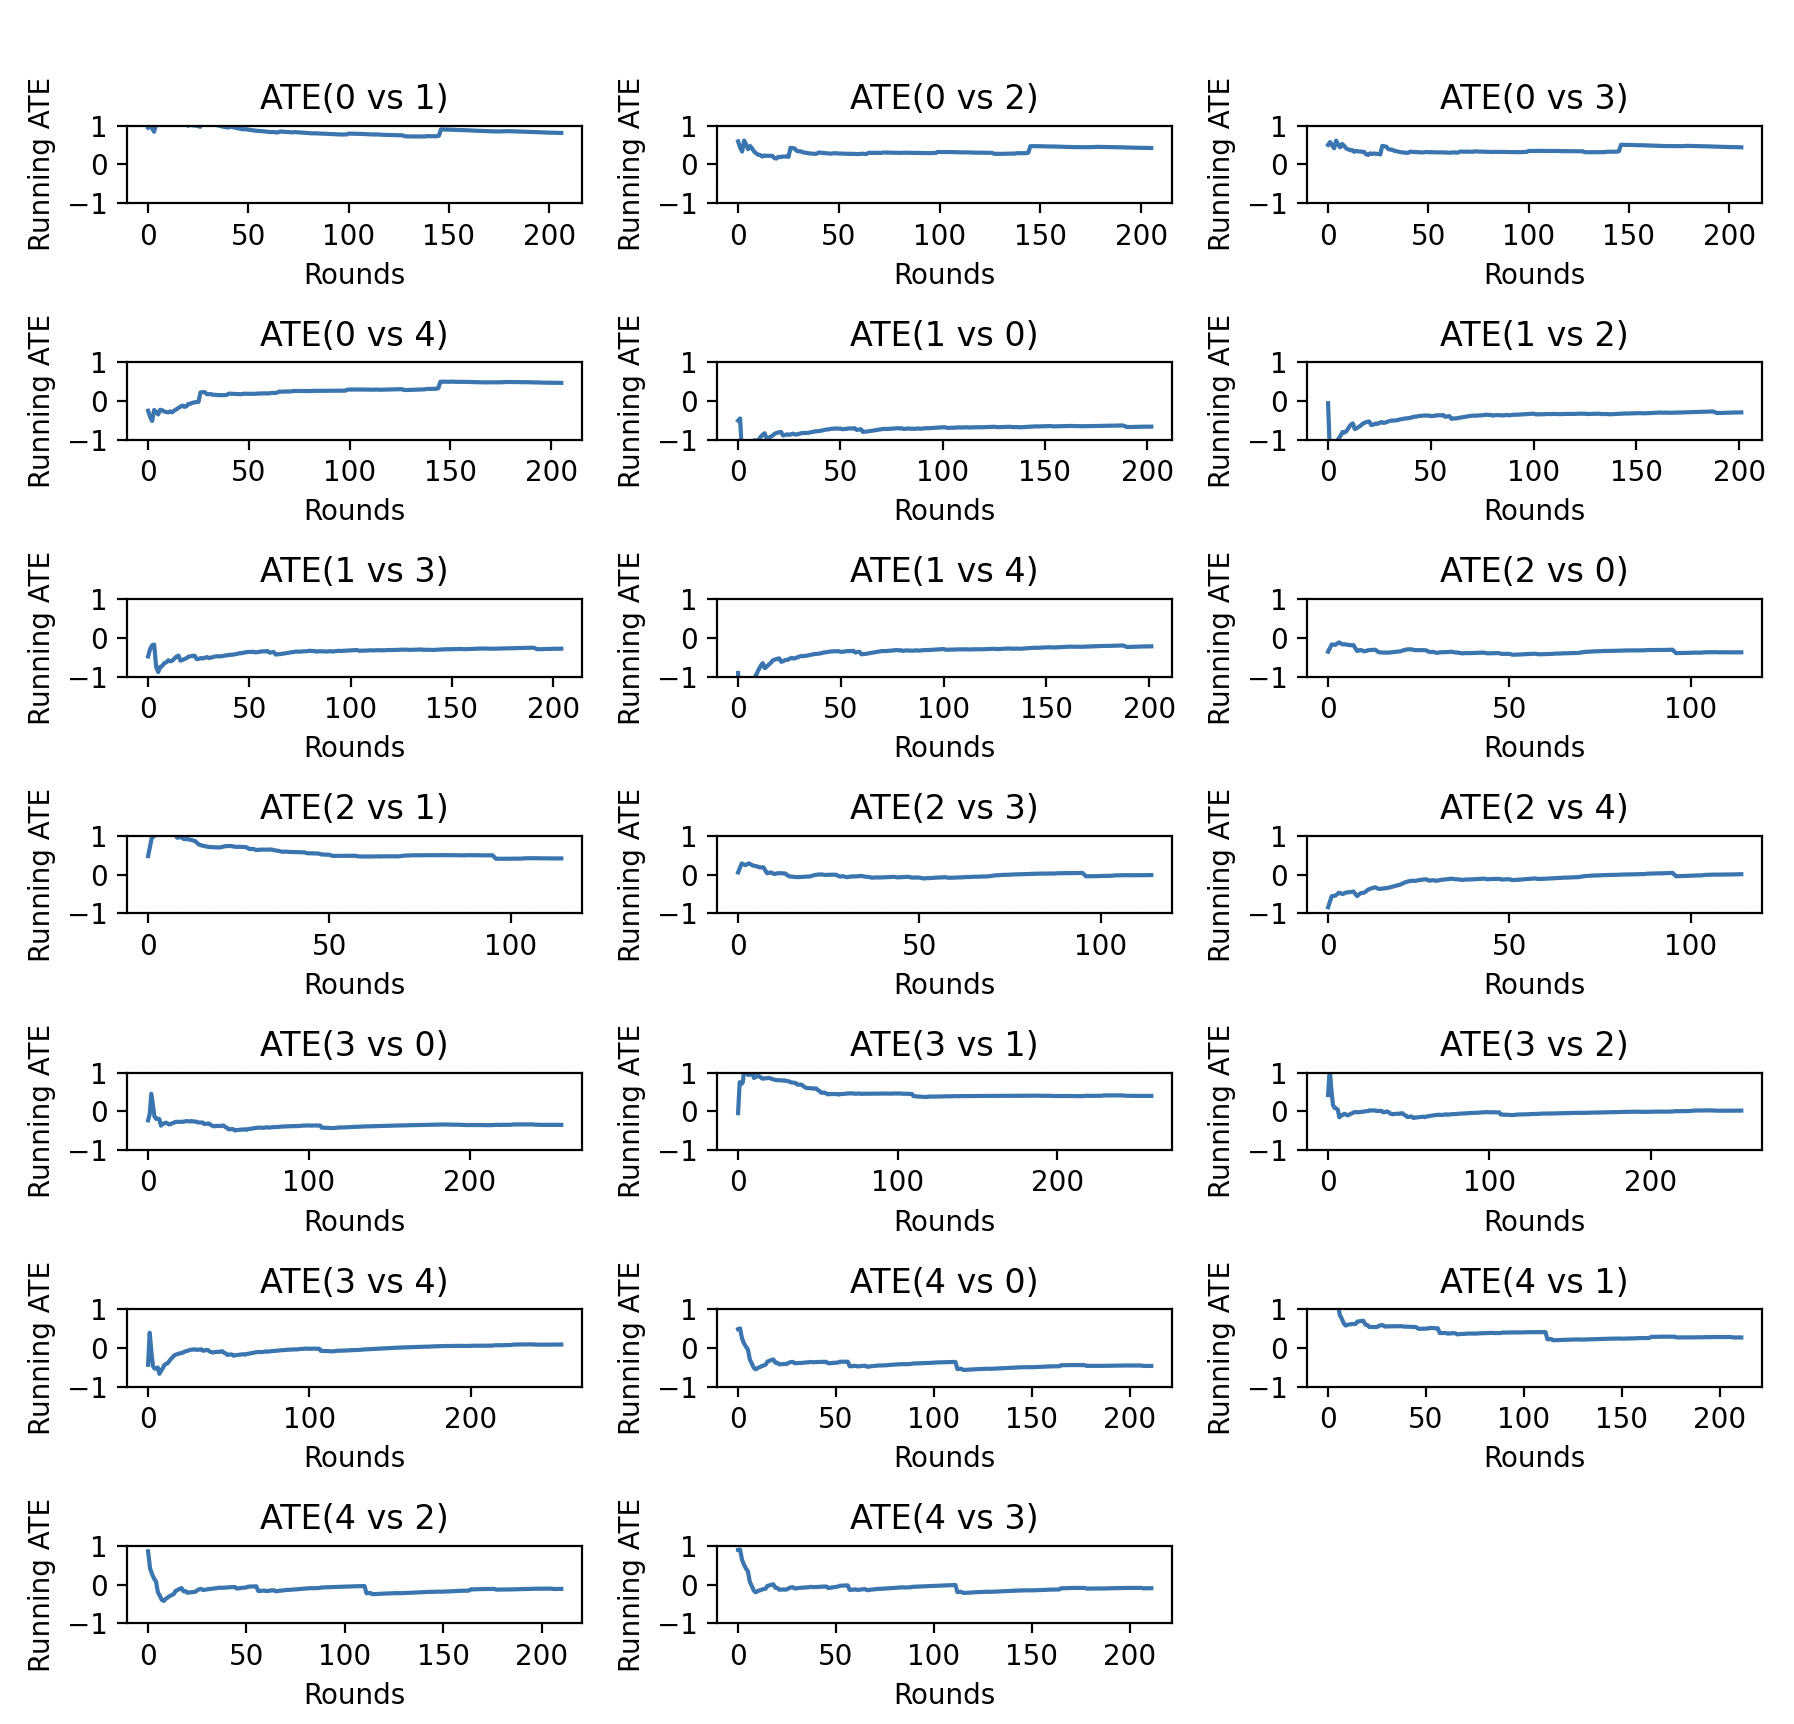
\includegraphics[width=0.9\textwidth]{ATE_with_IPW.png}
\caption{ATE Estimation Convergence for All Arm Pairs with IPW}
\label{fig:ate_pairs}
\end{figure}

Figure~\ref{fig:ate_pairs} demonstrates convergence of pairwise ATE estimates using inverse propensity weighting. Each subplot shows the running average of the difference between the selected arm and another arm’s IPW-adjusted reward. These plots confirm that ATE estimates stabilize over time, indicating the consistency of the estimator.

\begin{figure}[H]
\centering
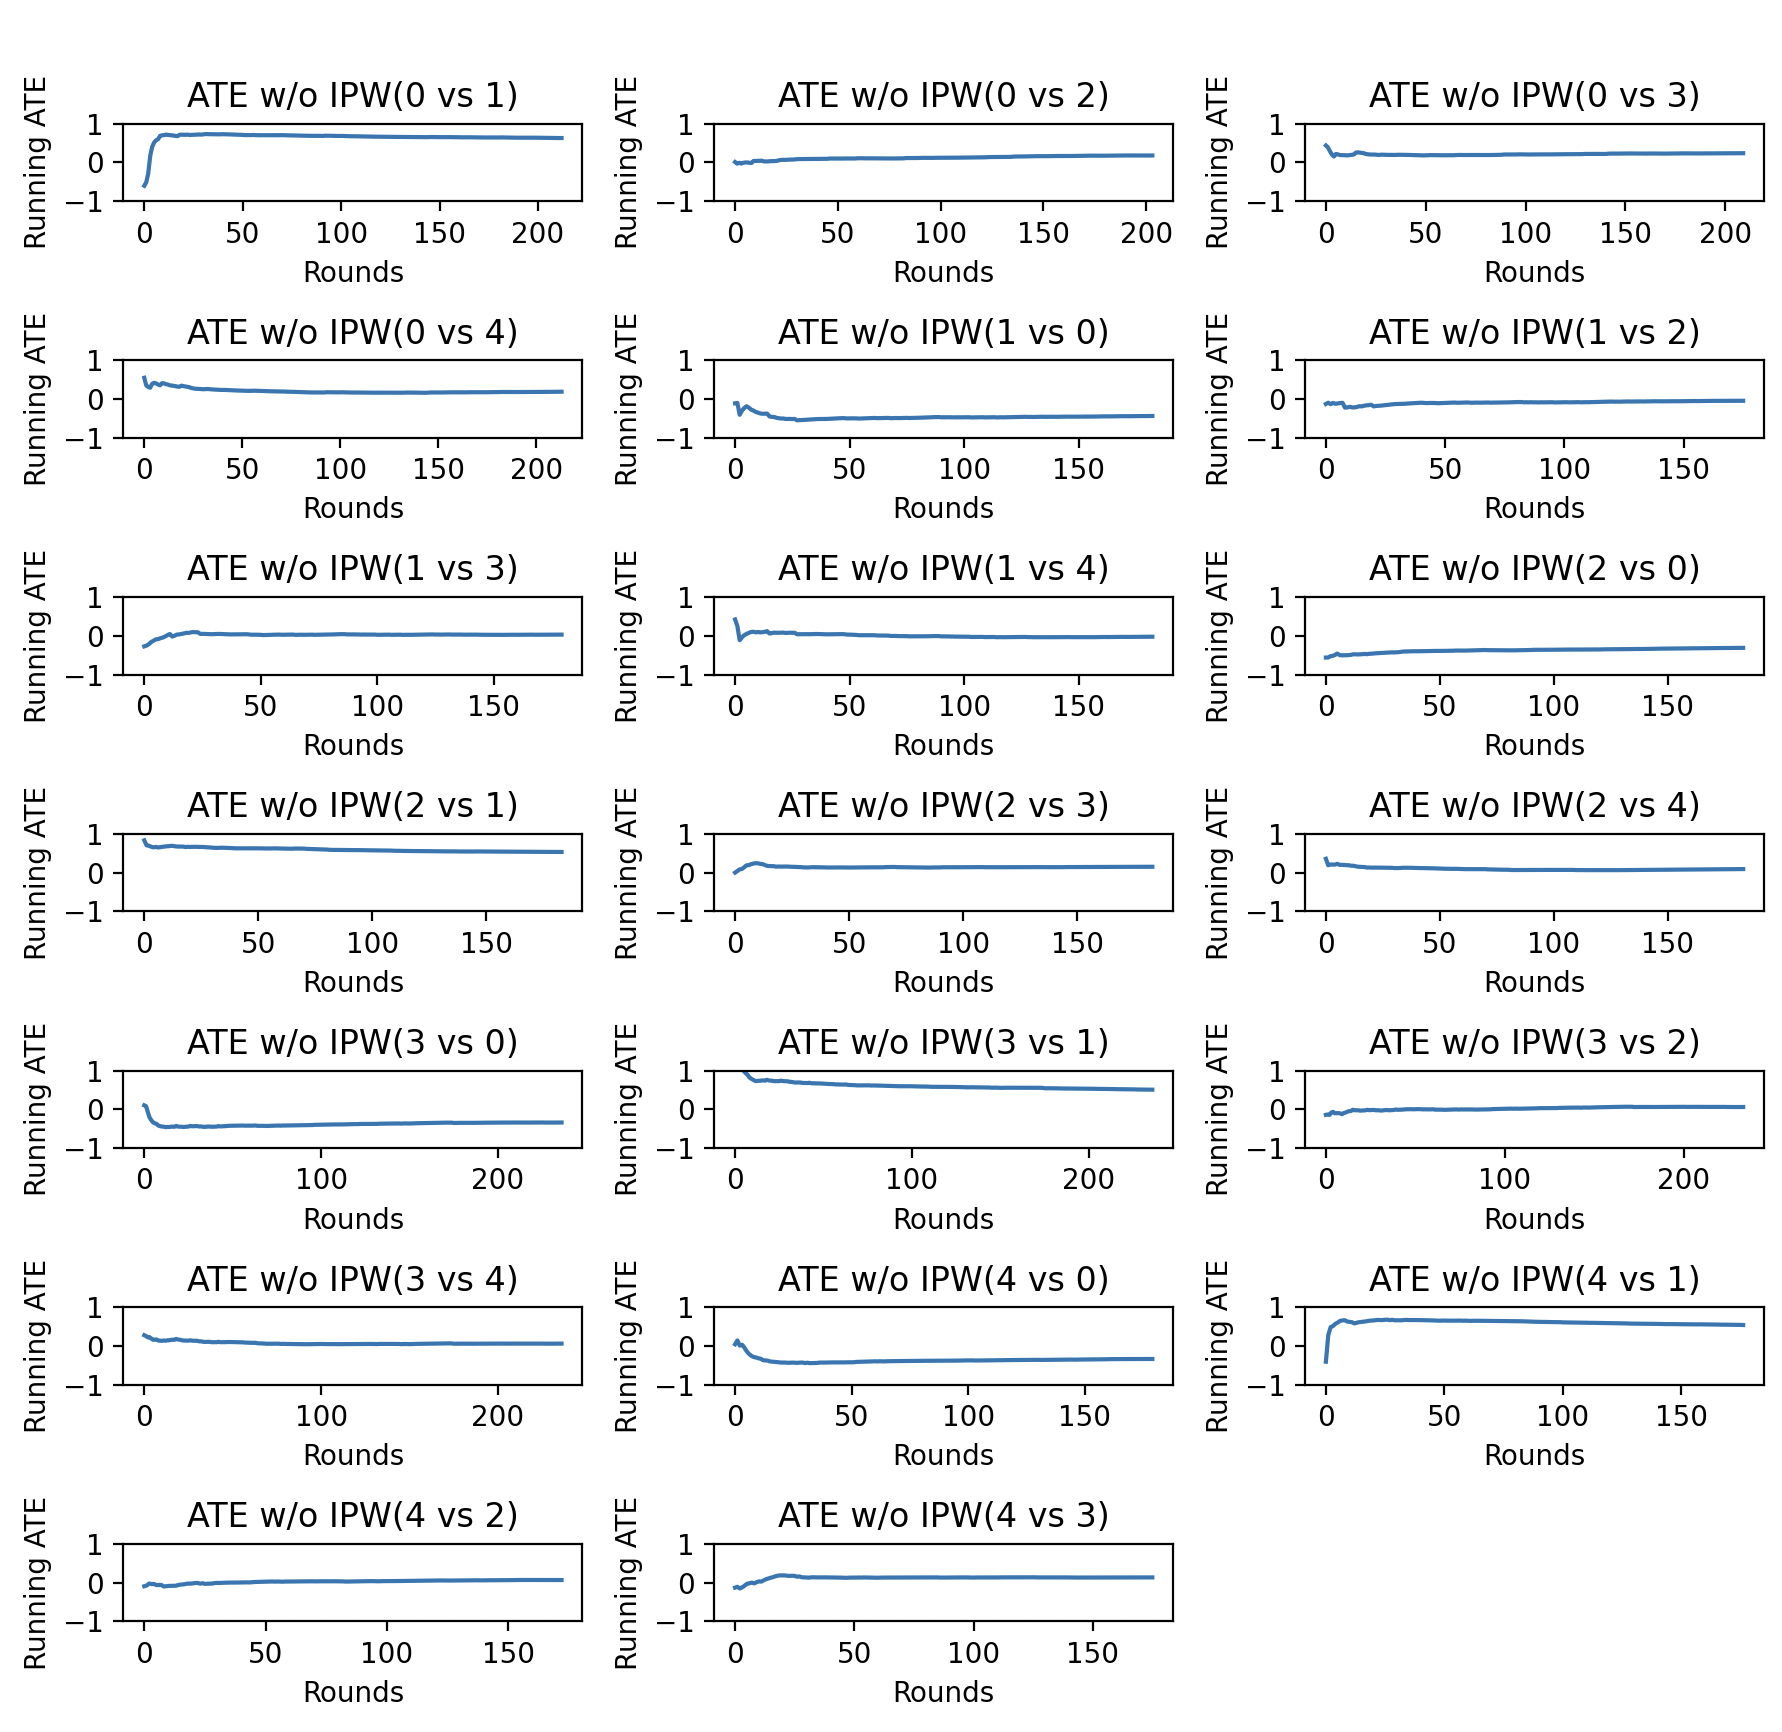
\includegraphics[width=0.9\textwidth]{ATE_without_IPW.png}
\caption{ATE Estimation Convergence for All Arm Pairs without IPW}
\label{fig:ate_pairs_no_ipw}
\end{figure}

Figure~\ref{fig:ate_pairs_no_ipw} demonstrates convergence of pairwise ATE estimates without using inverse propensity weighting. The subplots show the running average of the difference between the selected arm and another arm’s reward.

These experimental results show that LinEXP3E indeed effectively balances exploration and exploitation, as evidenced by sublinear cumulative regret and increasing average reward over time. Furthermore, the convergence of ATE estimates demonstrates the algorithm’s robustness for inference in a bandit setting. These findings empirically validate the theoretical motivations discussed earlier and underscore the advantages of incorporating both ATE \ref{eq:ATE} and regret \ref{eq:regret} into bandit-based learning and evaluation frameworks.